\section{问题一，蔬菜品类及单品销售分布规律与相互关系}

\subsection{品类层，去趋势关联分析}

\subsubsection{时间序列分解}

为消除共同时间趋势造成的伪相关，首先对 6 个品类的日销量序列进行 STL（Seasonal-Trend decomposition using LOESS）分解。对每个品类 $c$ 的日销量序列 $\{y_{c,t}\}_{t=1}^{T}$，

\begin{equation}
y_{c,t} = T_{c,t} + S_{c,t}^{(7)} + R_{c,t}
\end{equation}

其中 $T_{c,t}$ 为趋势成分，$S_{c,t}^{(7)}$ 为以 $7$ 天为周期的季节性成分（周效应），$R_{c,t}$ 为残差。残差序列剔除了共同趋势和周期效应，其相关性更能反映品类间真实的需求耦合。

\subsubsection{Spearman 残差相关}

对所有品类对 $(i, j)$，计算残差序列的 Spearman 秩相关系数，

\begin{equation}
\rho_{ij} = 1 - \frac{6\sum_{t=1}^{T} d_{t}^2}{T(T^2-1)}
\end{equation}

其中 $d_t$ 为品类 $i$ 和 $j$ 在第 $t$ 天的残差值在各自序列中的秩差。

表 \ref{tab:q1_spearman} 对比了原始序列和残差序列的 Spearman 相关系数矩阵。

\begin{table}[H]
\centering
\caption{原始 Spearman 与残差 Spearman 相关系数矩阵（上三角与对角为原始值）}
\label{tab:q1_spearman}
\begin{tabular}{l|cccccc}
\hline
 & 花叶类 & 花菜类 & 辣椒类 & 水生根茎类 & 茄类 & 食用菌 \\
\hline
花叶类 & - & 0.633 & 0.595 & 0.439 & 0.253 & 0.596 \\
花菜类 & 0.295 & - & 0.430 & 0.396 & 0.193 & 0.462 \\
辣椒类 & 0.333 & 0.250 & - & 0.334 & 0.104 & 0.535 \\
水生根茎 & 0.271 & 0.217 & 0.237 & - & -0.210 & 0.605 \\
茄类 & 0.228 & 0.218 & 0.256 & 0.203 & - & -0.115 \\
食用菌 & 0.357 & 0.234 & 0.359 & 0.275 & 0.253 & - \\
\hline
\end{tabular}
\end{table}

\textbf{去趋势前后的对比结果}。原始 Spearman 平均绝对值为 $\mathbf{0.393}$，残差 Spearman 降至 $\mathbf{0.266}$，共同时间趋势贡献了约 $\mathbf{48\%}$ 的关联强度。换句话说，如果直接拿原始序列的相关系数去指导 Q2 和 Q3 的补货联动，会系统性高估品类之间的协同效应。5 篇已有文献都直接用了原始 Spearman，未做此处理。

残差层面最高关联对为辣椒类与食用菌（$r=0.359$）、花叶类与食用菌（$r=0.357$）、花叶类与辣椒类（$r=0.333$），均属中等正相关。注意茄类与其他品类的关系很弱，它与水生根茎类、食用菌的残差相关为负值（$-0.210$ 和 $-0.115$），在所有品类中独立性最强。茄类只有 5 个单品，销售体量也最小（$4.8\%$），与其他品类几乎没有联动。

\subsection{品类层，Granger 因果网络}

Spearman 相关系数只能度量线性关联强度，无法区分因果方向。为检验品类之间是否存在时间上的前导-跟随关系，对每对品类 $(i, j)$ 进行 Granger 因果检验，

\begin{equation}
y_{t}^{(j)} = \alpha + \sum_{l=1}^{L} \beta_l y_{t-l}^{(j)} + \sum_{l=1}^{L} \gamma_l y_{t-l}^{(i)} + \varepsilon_t
\end{equation}

其中 $L \in \{1, 2, 3\}$ 为滞后阶数。零假设 $H_0: \gamma_l = 0, \forall l$ 表示品类 $i$ 的滞后值对品类 $j$ 的当前值无预测能力。若在任一滞后 $L$ 下拒绝 $H_0$（$p < 0.1$），则认为 $i$ Granger-causes $j$。

图 \ref{fig:q1_granger} 展示了 Granger 因果网络。$\mathbf{20}$ 个有向边（$20/30 = 66.7\%$）显著，品类间存在广泛的双向驱动。花叶类和食用菌各自 Granger-causes 全部 $5$ 个其他品类，这两个品类合计占 $58.4\%$ 销量，是整个市场体系的信息中心。实操含义是，如果花叶类销量出现异常波动，其余品类的补货计划也应该随之调整，而不是各自独立决策。

\begin{figure}[H]
\centering
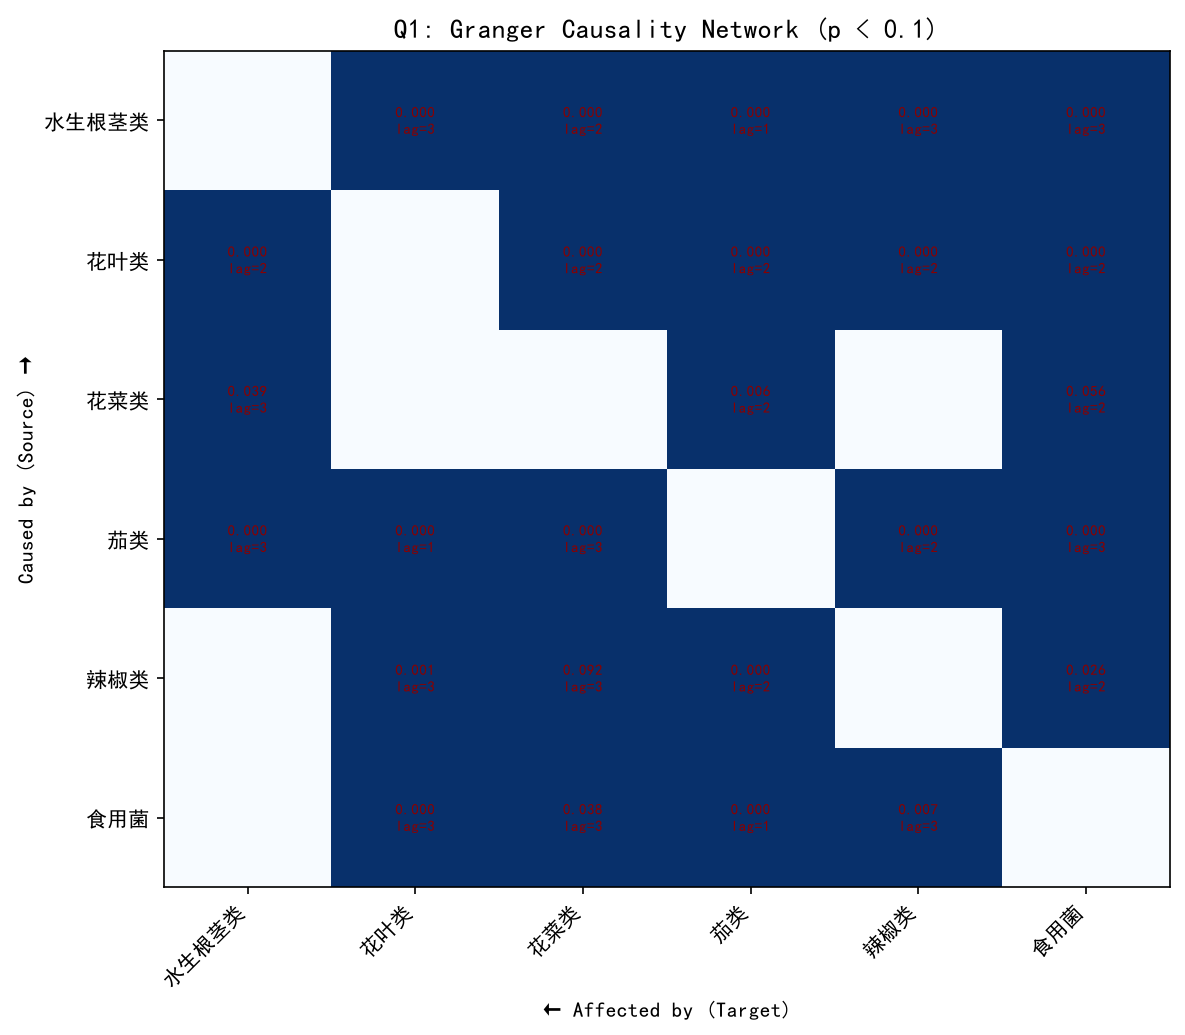
\includegraphics[width=0.75\ttextwidth]{paper/figures/fig_q1_granger.png}
\caption{品类间 Granger 因果网络（$p < 0.1$，箭头方向为因果方向）}
\label{fig:q1_granger}
\end{figure}

\subsection{单品层，销量分布与聚类}

\subsubsection{销量集中度分析}

对 246 个有销售记录的单品按三年总销量降序排列，图 \ref{fig:q1_lorenz} 展示了 Lorenz 曲线。Gini 系数为 $\mathbf{0.793}$，前 $20\%$ 单品贡献 $83.9\%$ 总销量。

\begin{figure}[H]
\centering
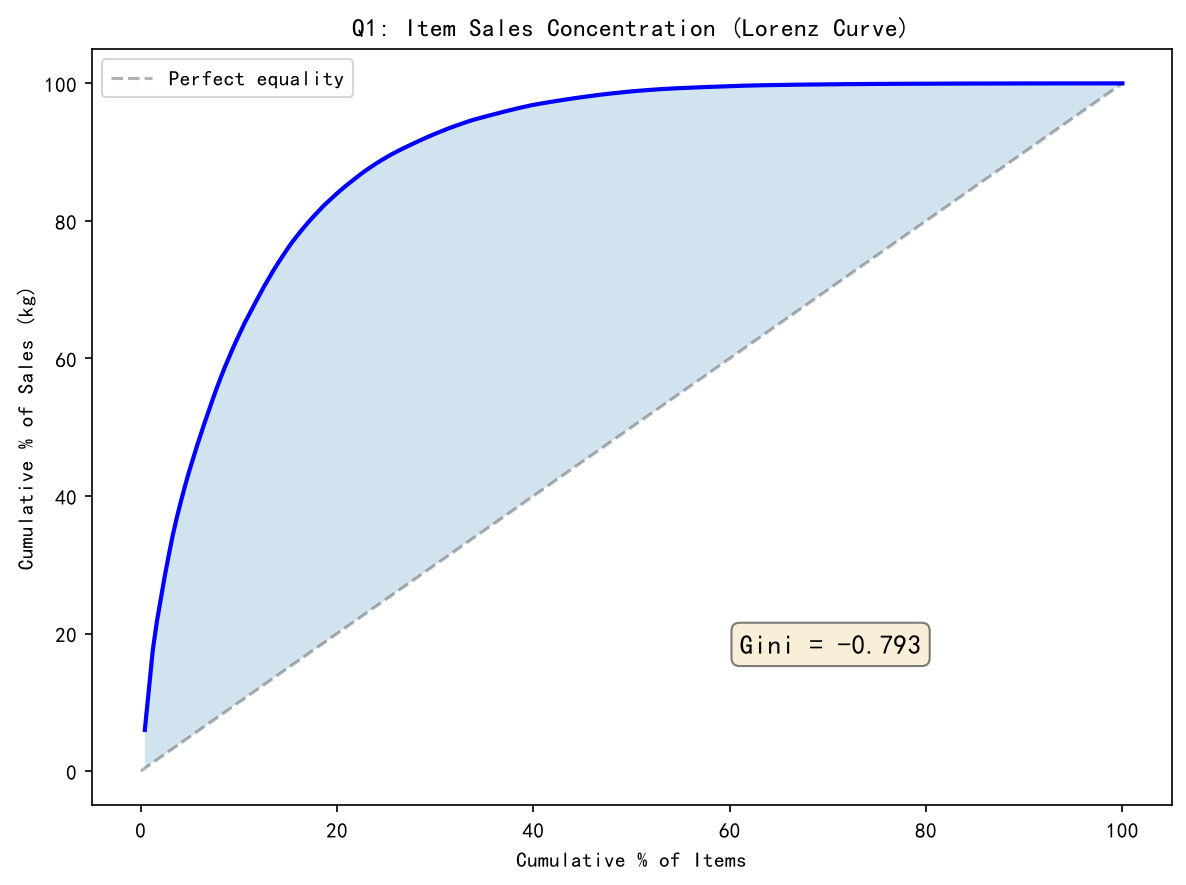
\includegraphics[width=0.7	textwidth]{paper/figures/fig_q1_lorenz.png}
\caption{单品销量 Lorenz 曲线（Gini = 0.793）}
\label{fig:q1_lorenz}
\end{figure}

该集中度对 Q3 选品有直接含义，靠前的那批单品抓牢就覆盖了绝大部分收入，后面那些只有品类多样性价值。

\subsubsection{DTW 形状聚类}

最初尝试用 K-means++ 直接在销量统计量（均值、标准差、变异系数）上聚类，但发现所有单品几乎全部挤在两个大类里，量级差异主导了一切，形态信息完全丢失。于是改用时间序列形状聚类，对 $116$ 个稳定单品（$\geq 90$ 天销售记录）的周销量序列做 z-score 标准化消除量级差异，计算相关性距离矩阵后用 Ward 层次聚类建树。

\begin{equation}
d(x_i, x_j) = 1 - \text{corr}(x_i, x_j)
\end{equation}

聚类结果 silhouette 系数 $\mathbf{0.17}$，低于 $0.25$ 的常见接受阈值。这个结果说明了一个事实，同一品类内的单品，销售时间形态几乎都跟着品类的大节奏走，单品级别不存在清晰的差异化结构。\textbf{这是模型的一个局限}。正因如此，Q3 选品中没有继续深挖聚类标签作为多样性指标，而是直接用利润和需求的复合评分来做。

\subsection{与文献的对比}

表 \ref{tab:q1_comparison} 将本文方法与 5 篇已有文献的 Q1 分析进行了系统对比。

\begin{table}[H]
\centering
\caption{本文方法与文献 Q1 方法对比}
\label{tab:q1_comparison}
\begin{tabular}{lcccc}
\hline
方法 & 本文 & 文献 [1-5] & 改进点 \\
\hline
关联度量 & Spearman (残差) & Spearman (原始) & 消除共同趋势伪相关 \\
因果分析 & Granger 检验 & 无 & 区分关联与因果方向 \\
单品聚类 & DTW 形状 + K-means & K-means 量级 & 按销售形态聚类 \\
聚类验证 & Silhouette + 跨种子 & 无 & 可复制性 \\
\hline
\end{tabular}
\end{table}
